
%%%DOCUMENTCLASS%%%
\documentclass[a4paper, 12pt, english, fleqn]{article}


%%%USEPACKAGES%%%
\usepackage[utf8]{inputenc}
\usepackage{babel}
\usepackage{coordsys,logsys,color}
\usepackage{fancyhdr}
\usepackage{hyperref}
\usepackage{texdraw}				
\usepackage[T1]{fontenc}					
\usepackage{amsmath,amsfonts,amssymb}	
\usepackage[normalem]{ulem}	
\usepackage{listings}
\usepackage{graphicx}
\usepackage{enumitem}
\usepackage{caption}
\usepackage{wrapfig}

%%%PAGESTYLE%%%
\pagestyle{fancy}

%%%CAPTIOBSETUP%%%
\captionsetup[figure]{font=small,labelfont=small,skip=3pt}

%%%LINKING%%%
\hypersetup{colorlinks=true, breaklinks=true, linkcolor=blue, menucolor=darkred, urlcolor=darkblue, citecolor=darkblue}

%%%NEWLIST%%%  
\newlist{aims}{enumerate}{1}
\setlist[aims,1]{
  label={Aim~\arabic*},
  leftmargin=*,
  align=left,
  %labelsep=1mm,
  font=\bfseries
}

%%%NEWCOMMAND%%%
\newcommand{\titlefont}[1]{\textcolor{black}{\fontseries{bx}\fontshape{n}\fontsize{30}{0pt} \selectfont #1}}
\newcommand{\titlepagef}[1]{\textcolor{black}{\fontseries{bx}\fontshape{n}\fontsize{14}{0pt} \selectfont #1}}
\newcommand{\gloss}[1]{\textcolor{glossb}{\fontsize{11}{0pt}\selectfont #1}}
\newcommand{\spaceline}[1][8pt]{\vskip #1}
\newcommand{\attrname}[1]{\textcolor{fgcgray}{\scriptsize #1}}
\newcommand{\comment}[1]{\spaceline[5pt] \textcolor{fgcgray}{\scriptsize #1} \spaceline[15pt]}


%%%RENEWCOMMAND%%%
\renewcommand{\familydefault}{cmss}


%%%DEFINECOLOR%%%
\definecolor{fgcgray}{rgb}{0.4, 0.4, 0.4}
\definecolor{darkred}{rgb}{.6,0,0}
\definecolor{glossb}{rgb}{0,0,0.38}


%%%LENGTH SETTINGS%%%
\addtolength{\oddsidemargin}{-1.0cm}
\addtolength{\evensidemargin}{-1.0cm}
\addtolength{\headwidth}{2.0cm}
\addtolength{\textwidth}{2.0cm}

\setlength{\parindent}{0cm}


%%%DEFINITIONS%%%
%Füge Überschriften ein
%Füge Namen ein

\makeatletter

\def\@maketitle{
  %\begin{titlepage}
   
  \begin{center}
      \titlepagef{Software-Project 2017}
      \spaceline
  \end{center}
  
  \begin{center}
      \parbox{\textwidth}{
        \spaceline
        \centering{\titlefont{\@title}}
        \par
        \spaceline
      }
  \end{center}
  
  \begin{center}
    \titlepagef{Real-Time Mesh Utilities}
    \spaceline[2em]
  \end{center}
  
  \begin{center}
  \begin{tabbing}
	Simon Heinke \qquad \=
	Julius Lerm \qquad \=
	Felix Griesau \qquad \=
	Marco Klamke \\
	Lars Debor
	\>Petros Simidyan
	\>Blerta Hamzallari
	\>Sugandha Sachdeva
  \end{tabbing}
  \end{center}
 
  \spaceline[3em] {
    \begin{flushright}
    \begin{tabular}[t]{rl}
      \attrname{last Change:} & \@date
    \end{tabular}
    \end{flushright}
    \par
  }
  \spaceline[5.5em]
  %\end{titlepage}
}

\makeatother


\begin{document}
  
  \pagenumbering{gobble}

  \lhead{\sc{Functional Specification}}

\title{Titel}

\vspace{3 in}

\maketitle \clearpage
  \pagenumbering{arabic}

\section{Introduction}

	Medicine today is highly advanced and is able to treat an immense amount of diseases and disorders.
	This results in high standards and a lot of pressure on people working in this branch. In order to further improve the 			standards the amount of errors has to be minimized, since they can have fatal consequences. %TODO siehe Feedback

	In pursuance of achieving, maintaining as well as improving these abilities, technological assistance is of utmost 				importance.\\  

	Since the brain is one of the main organs, caution and accuracy is essential while treating its conditions. 
	
	Techniques such as the MEG (Magnetoencephalography) or EEG (Electroencephalography) observe the brains activity by 				measuring and monitoring magnetic fields or electrical deviations produced by groups of neurons.

	These procedures help diagnosing epilepsy, migraine variants and other brain diseases. In addition, assistance in 				research and localization of epilepsy is one possible usage of EEG/MEG. 
	 
	Furthermore they are used for research in fields like psychology.
	A proper visualization aids the usability of generated data and provides a superficial graphic overview of the brains 			activity, thus enabling first interpretations or even diagnosis.\\
	

	The MNE-CPP  project builds tools for the purpose of making the analysis of EEG and MEG data easier.
	Thus, the whole project is open-source and everyone can contribute. As programming language only C++ is used, although the 	project simultaneously exists in other languages, e.g. Python. 
	MNE Scan, Analyze and Browse are some of the standalone features of the existing framework. \\

	The new extension of the current project focuses on real-time 3D-visualization of EEG/MEG sensor data, while being as 			exact and fast as possible. It should both be integrated into the existing code and accessible through MNE Scan, which 			functions as the real-time acquisition and processing software in the MNE-CPP project. MNE-CPP and thus MNE Scan are cross 	platform capable (Windows, Linux, Mac). 
  
\clearpage
  \tableofcontents \clearpage
  
  \section{Requirements} 

	The product receives EEG/MEG sensor data and constructs a real-time 3D visualization of the brains current activity.
	Users can choose between further options, changing the output immediately to their personal preferences. 

\subsection{Mandatory criteria}

	The following functions have to be implemented correctly and must fulfill given requirements.
		
\subsubsection{Surface constrained distance calculation (Geodesic problem on meshes)} \label{scdc}
	%Abkürzung SCDC einführen
	Because the brain has an uneven surface, a function for calculating the distance between two separate points is needed.
	
	As the euclidian distance would not respect the structure of the surface, a different approach for determining the exact 	distances has to be implemented.  
	The function receives input data in form of a preprocessed triangulated surface mesh and calculates the distance between 	the vertices.			

	\begin{aims}
	
		\item[C111] Based on that data, the function calculates a matrix that holds values describing the distances between 						all vertices using double precision. 
		\item[C112] The function must be able to process up to 200,000 vertices.
		\item[C113] The user can limit the calculation to a subset of vertices.
	
	\end{aims}

\subsubsection{Point to plane mapping}

	Since the sensors do not directly touch the head, therefore float slightly above it, an accurate projection is needed to 
	exactly localize their positions regarding the brain. 
	
	Hence a function must be implemented to solve this problem. 
	The function receives a set of sensor locations in 3D-Space and maps them onto the underlying surface mesh. Thus every 			sensor gets assigned to a vertex of the mesh. 

	\begin{aims}
	
		\item[C121] The function must be able to handle data from MEG-sensors which have a known orientation.
		\item[C122] The function must be able to handle data from EEG-sensors which are non-orientated.
	
	\end{aims}

\subsubsection{Interpolation algorithm} 

	The algorithm receives a mesh and a subset of vertices %todo von den letzteren auch die sensorwerte
	%todo Sensorwerte repraesentieren Gehirnaktivitaeten
	
	\begin{aims}
	
		\item[C131] Based on the said subset the algorithm must calculate the values for every vertex of the mesh.
		\item[C132] For this, the algorithm creates a matrix storing weights for the later interpolation.
					The interpolation process can be summarized by the following equation: 
					
					$y_{full} = W \cdot y_{sub}$
					, where $W$ is the mentioned matrix and $y_{sub}$ is the current dataset for the known sensors, i.e. 							vertices.
		\item[C133] The calculation of the weight matrix must be based on the result of the SCDC (\ref{scdc}).
	
		%SCDC referenzieren
	
		%TODO Bad channels beachten
	
	\end{aims}

\subsubsection{Integration in Disp3D}
	In order to ensure usability within the given framework MNE-CPP, the final visualization must be integrated into the 			preexisting GUI, namely Disp3D.
	
	\begin{aims}
		
		\item[C141] A new function must be added to the Disp3D tree model. Internally this function must create a new 								handler.%todo Lorenz fragen, weil satz im Lastenheft nicht von dieser Welt.
		
		%todo in scan einfuegen nicht gleich disp3D
	\end{aims}
	
\subsection{Non-Functional Requirements}
	
	%todo Klassen-/Methodennamen, Windows/Linux Unterstützung	
	
	%todo Graka-Matrizen-Shice
	
	%todo fancy product video apple style
	
	\begin{aims}

		\item[C211] The software has to run on the latest versions of 2 operating systems, namely Windows and Linux.%vll nur Ubuntu?
		%todo ueberlegen, ob das vielleicht besser nur in Product environment steht
	
	\end{aims}
	
\subsection{Optional criteria}
	
	Besides of the mandatory features there is some functionality that would enrich the software but are not set as main goals.  %Einfuehrung einige Features wuenschenswert...evtl umformulierung...
	
\subsubsection{SCDC}
	
	\begin{aims}
		
		\item[C311] The computation time should not exceed 1 second.
			
	\end{aims}
	
\subsubsection{Interpolation}

	\begin{aims}
	
		\item[C321] One interpolation cycle should take less than 17ms.
		\item[C322] Multiple methods for calculating the weight matrix can be implemented. The user can select one.
	
	\end{aims}
	
	
\subsection{Differentiating criteria}
	
	\begin{aims}
		
		\item[C411] The program receives preprocessed data and does get in touch with hardware sensors.
		\item[C412] The program does not evaluate the data but processes the data for further visualisation. %bereitet nur daten fuer die visualisierung auf, inhaltlich wird erstmal nichts 							interpreitert
	
	\end{aims}
	



	
 \clearpage
  %\section{Produkteinsatz}
Zur Beantwortung der Frage, was das System unter welchen Rahmenbedingungen leisten soll, werden Anwendungsbereich, Zielgruppe und Betriebsbedingungen spezifisch betrachtet.
\subsection{Anwendungsbereich}
Die Anwendung wird dort zum Einsatz kommen, wo der Transfer von Daten eine wichtige Voraussetzung für das Arbeiten an teilweise stark verstreuten Standorten darstellt.
Dabei spielt insbesondere die effiziente, verschlüsselte und sichere Übertragung, welche für riesige Datenmassen mit den herkömmlichen Methoden nur schwer umzusetzen ist, eine große Rolle.
Mit dem System wird versucht, die Verschlüsselung von Ethernet-Rahmen nahezu in Echtzeit zu ermöglichen.

\subsection{Zielgruppe}
Im Allgemeinen ist die gebotene Funktionalität für alle interessant, die große Massen an Daten, zwischen nicht direkt verbundenen Netzwerken über ein nicht vertrauenswürdiges Netz verschlüsselt übertragen wollen. 
Insbesondere kann dies für diverse Unternehmen, Behörden oder auch NGOs (Non-Governmental Organisations) nützlich sein, die organisationsintern große Datenmassen besonders schnell und sicher transferieren müssen.


\subsection{Betriebsbedingungen}
Um die Verschlüsselung von Ethernet-Rahmen in nahezu Echtzeit umzusetzen, kommt das \gloss{DPDK} zum Einsatz. 
Dieses ermöglicht Pakete direkt in den Hauptspeicher des Rechners zu übertragen, ohne Interruptlast zu erzeugen.
Für die Umsetzung des Verschlüsselungsverfahrens verwendet das System \gloss{AES}, wobei die Verschlüsselung durch Zuhilfenahme von \gloss{AES-NI} beschleunigt wird.
Bei langfristiger Nutzung des Systems wird versucht hohe Stabilität zu gewährleisten, damit eine wartungsfreie Laufzeit ermöglicht wird.
 \clearpage
  %\section{Produktumgebung}
Zur Beschreibung der Produktumgebung wird im Folgenden die Netzwerktopologie und ein Szenario betrachtet. Insbesondere werden auch die Voraussetzungen an Hardware und Software genauer beleuchtet.

\subsection{Szenario}
Abbildung 1 soll das im Folgenden geschilderte Szenario verbildlichen.

Wie bereits beschrieben, handelt es sich bei PECTO um ein Encryption-Framework, welches den effizienten und verschlüsselten Datenaustausch zwischen einzelnen \gloss{roten Netzen} durch ein \gloss{schwarzes Netz} ermöglicht.
Ein \gloss{rotes Netz} besteht aus einem physischen, durch Ethernet verbundenen Netzwerk, dass von einer Instanz des Systems geschützt wird.
Das \gloss{schwarze Netz} trennt mehrere verschiedene \gloss{rote Netze} voneinander.
Dabei agiert jede Instanz als Schnittstelle zwischen dem \gloss{schwarzen} und einem \gloss{roten Netz}.
Mehrere Instanzen bilden eine Gruppe, wenn sie die gleiche Netzgruppe schützen.
Eine Netzgruppe besteht dabei aus mehreren physisch getrennten \gloss{roten Netzen}, die logisch ein großes Netzwerk bilden.
Verschiedene Gruppen können zwar koexistieren, jedoch nicht miteinander kommunizieren.
Möchte nun eine Einheit aus einem roten Netz mit einer anderen aus einem zweiten roten Netz derselben Gruppe kommunizieren, werden die Daten an die für das Netz zuständige Instanz geleitet, welche Verschlüsselung und Weiterleitung übernimmt.
Kommt das Paket bei der anderen Instanz an, wird dieses, wie in den Zielbestimmungen beschrieben, klassifiziert und ggf. im dortigen roten Netz zur Zieladresse geschickt.     
 
  \begin{figure}  
    \begin{center}
	  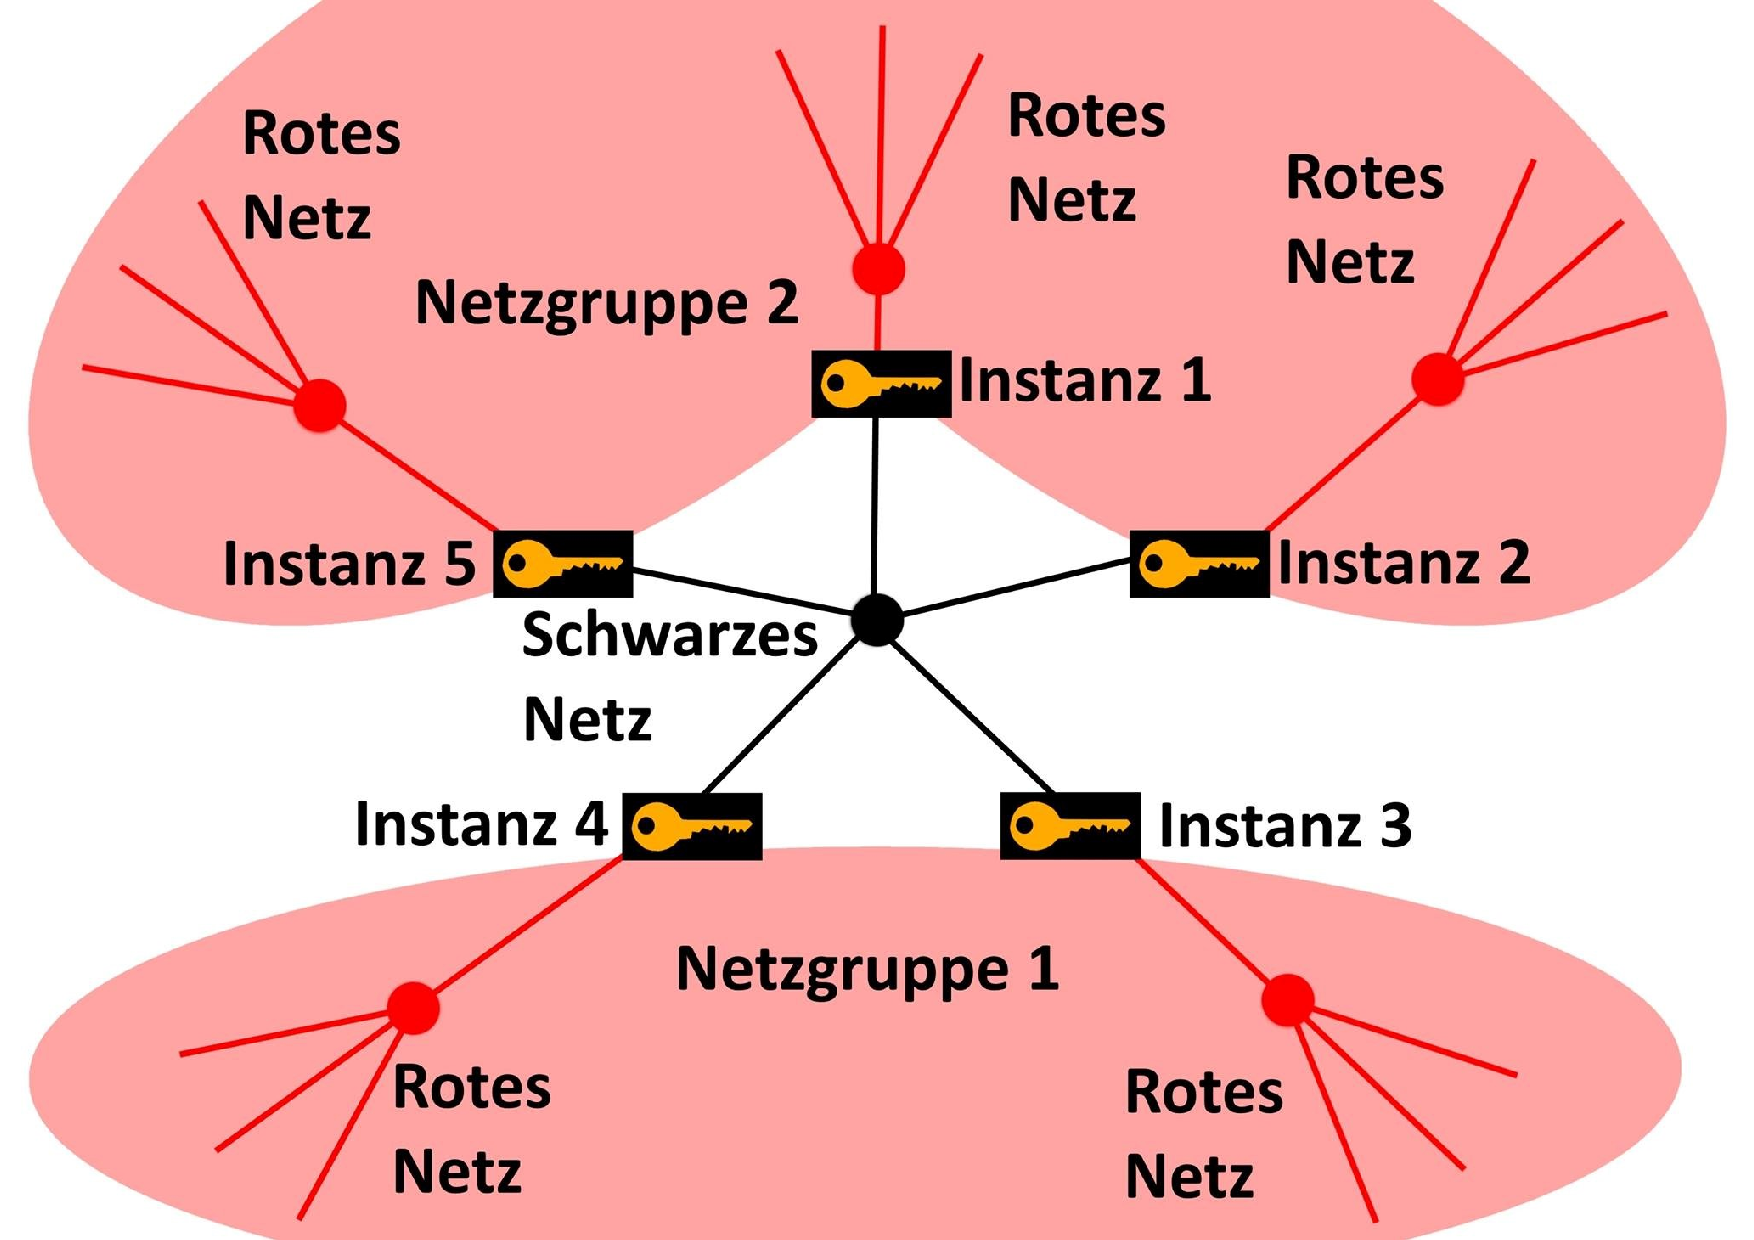
\includegraphics[width = 10cm]{Bilder/PECTO_Skizze.pdf}
	  \caption{Aufbau des Systems}
    \end{center}
  \end{figure}  
  
  
\subsection{Software}
Das System wird auf Linux-basierenden Bertriebssystemen lauffähig sein.

Eine Kerntechnologie, die genutzt wird um, die Anforderungen an dieses System angemessen umzusetzen, ist Intel's Data Plane Developement Kit (\gloss{DPDK}). 
Dieses Framework ermöglicht den direkten Zugriff aus dem Userspace auf die Netzwerkkarte. Es bietet zudem die Möglichkeit Pakete direkt in den Hauptspeicher des Rechners zu übertragen, ohne Interruptlast zu erzeugen. 
Für die erleichterte Bedienung wird eine Hardwareabstraktionsschicht (\gloss{EAL}) erzeugt, welche den Zugang auf Teile der Hardware des Linux-Kerns, durch Klassen, Methoden und Funktionen erlaubt.
Ein einfacherer Zugriff auf den Data-Link-Layer und Möglichkeiten zur schnellen Weiterleitung lassen sich durch erweiterbare Funktionen des Framework realisieren.
Zusätzliche hierzu bietet das \gloss{DPDK} auch noch eine Reihe von anderen Funktionen, welche für die Verschlüsselung, basierend auf \gloss{AES}, das Authentifizieren, dem Packet-Forwarding und der Schlüsselaushandlung genutzt werden.

\subsection{Hardware}

Das System soll Architekturen auf x64-Basis unterstützen. 
Um lauffähig zu sein, benötigt es außerdem \gloss{DPDK}-kompatible Netzwerkkarten und einen Prozessor, welcher die Nutzung von \gloss{AES-NI} möglich macht.
Zur Verwendung des Systems ist außerdem ein Zugang zu einem Ethernet-basierten Kommunikationskanal notwendig.
Dieser muss in der Lage sein, eine Übertragungsrate von bis zu 40 Gigabit/s zu realisieren.

\subsection{Netzwerktopologie}

Es gibt mehrere \gloss{rote Netze}, die zu einer Netzgruppe gehören, aber nicht direkt miteinander verbunden sind.
Alle Clients der Netzgruppe verwenden die gleiche Subnetzmaske.
Das \gloss{schwarze Netz} trennt die einzelnen \gloss{roten Netze}. 
Dabei ist die Topologie, welche im \gloss{schwarzen Netz} vorliegt, für das System unbedeutend.
Die Instanzen des Systems agieren lediglich als Übergang zwischen dem \gloss{schwarzen} und den \gloss{roten Netzen}.
Es wirkt nach außen hin wie ein \gloss{Layer-2-Switch}, welcher die Weiterleitung der Datenpakete auf dem Data-Link-Layer übernimmt. 







 \clearpage
  %\section{Product Functions}

\subsection{User Functions}

	\begin{aims}
	
		\item[F11] The user can access the implemented features as a part of MNE Scan (see section \ref{3_1_scope}).
		\item[F12] Either MEG or EEG data can be used as input.
		\item[F13] Any desired surface mesh and set of sensor data, selected by the user, can be used as input data for 							further calculations.
		\item[F14] A preferred subset of vertices can be selected, to perform distance calculations on. 
		\item[F15] The user is able to select a threshold for identifying all relevant vertices while interpolating. 
		\item[F16] As part of MNE Scan/Disp3D all graphical options are available to the user, meaning e.g. different 								coloring and rotation of the object.
	
	\end{aims}

\subsection{Offline Functions}
	
	These functions are performed one time and are executed prior to the interpolation process.	
	
	\begin{aims}
	
		\item[F21]	The distance between two vertices on a given mesh, is calculated following the structure of the surface. 						Therefore the euclidian distance is not used.
		\item[F22] All floating sensor points are projected onto the nearest vertices on the input mesh. 
		\item[F23] A weight matrix, containing values for all vertices, is generated. 
 	
	\end{aims}
	
\subsection{Real-Time Functions}

	These functions are performed continuously and in real-time.	
	
	\begin{aims}
	
		\item[F31]	Based off prior calculations, the interpolation assigns every vertex a value.
		%\item[F32] A visual output is generated. %TODO bleibt das so?
	
	\end{aims} \clearpage
  %\section{Produktdaten}

Die Punkte \textbf{D0XX} stellen die benötigten Datensätze dar. 
Diese Datensätze liegen im Normalfall zweimal vor, einmal auf der Zielinstanz (zur Verschlüsselung) und einmal auf der Senderinstanz (zur Entschlüsselung).
\begin{description}
  \item[D010]\textit{Schlüssel:} Der Schlüssel mit dem die Pakete verschlüsselt werden.
  \item[D020]\textit{Sequenznummern:} Versandte Pakete werden durch einen definierten Zähler nummeriert.
  Dieser ist zu Beginn des Initalisierungsvektors, welcher aus dem zugeteilten \gloss{IV-Space} generiert wird, definiert. 
  Somit kann gewährleistet werden, dass die Instanzen unterschiedliche Intialisierungsvektoren verwenden.
  Nummerierung der gesendeten Pakete durch einen definierten Zähler zu Beginn der Initialisierungsvektoren im zugeteilten \gloss{IV-Space}.
  \item[D030]\textit{Forwarding-Tabellen:} Die Forwarding-Tabelle einer Instanz enthält die IP- und MAC-Adressen aller Rechner, welche sich in dem \gloss{roten Netz} befinden, für die diese Instanz zuständig ist. 
  Außerdem sind auch die IP-Adressbereiche, der \gloss{roten Netze}, für welche die anderen Instanzen verantwortlich sind, Teil der Tabelle.
  
\end{description} \clearpage
  %\section{Produktleistungen}

\begin{description}
	\item[L010]\textit{Wartungsfreiheit:} Das System soll, nachdem es eingerichtet worden ist, stabil arbeiten, ohne die Aufmerksamkeit des Nutzers zu fordern.
	\item[L020]\textit{Hoher Paketdurchsatz:} Das System soll eine sehr große Menge an Netzwerkpaketen verarbeiten können.
	\item[L030]\textit{Geringe Latenz:} Das System soll Pakete mit geringst möglicher Verzögerung übertragen.
	\item[L035]\textit{Jitter:} Das System soll Pakete mit der geringst möglichen Genauigkeitsschwankungen im Übertragungstakt(Chock) senden.
	\item[L040]\textit{\gloss{Robustheit:}} Das System soll auch unter ungünstigen Bedingungen, zum Beispiel in einem stark belasteten Netz, zuverlässig funktionieren.
	\item[L050]\textit{Recheneffizienz:} Das System soll möglichst effizient mit der vorhandenen Rechenleistung arbeiten.	
\end{description}



 \clearpage
  %\section{Benutzungsoberfläche}

Auf Grund der prinzipiellen Art der Anwendung des Systems kann auf ein Graphical User Interface (GUI) verzichtet werden.

  %\section{Qualitätszielbestimmungen}

\begin{center}
 \begin{tabular}{l|c|c|c|c}
  ~ & sehr wichtig & wichtig & weniger wichtig & unwichtig\\
  \hline \hline
  \gloss{Robustheit}~ &  ~ ~ ~ &  ~ $\surd$ ~ &  ~ ~ ~ &  ~ ~ ~ \\
  \hline
 \gloss{Zuverlässigkeit}~ &  ~ $\surd$ ~ &  ~ ~ ~ &  ~ ~ ~ &  ~ ~ ~ \\
  \hline
  Korrektheit~ &  ~ $\surd$ ~ &  ~ ~ ~ &  ~ ~ ~ &  ~ ~ ~ \\
  \hline
  \gloss{Benutzerfreundlichkeit}~ &  ~ ~ ~ &  ~ ~ ~ &  ~ ~ ~ &  ~ $\surd$ ~ \\
  \hline
  \gloss{Effizienz}~ &  ~ $\surd$ ~ &  ~ ~ ~ &  ~ ~ ~ &  ~ ~ ~ \\
  \hline
  \gloss{Portabilität}~ &  ~ ~ ~ &  ~ ~ ~ &  ~ ~ ~ &  ~ $\surd$ ~ \\
  \hline
  Kompatibilität~ &  ~ ~ ~ &  ~ ~ ~ &  ~ ~ ~ &  ~ $\surd$ ~ \\
  \hline
  \gloss{Sicherheit}~ & ~ $\surd$ ~ & ~ ~ ~ & ~ ~ ~ & ~ ~ ~ \\
 \end{tabular}
 
 
\end{center}
 \clearpage
  %\section{Testszenarien und Testfälle}


Die hier aufgeführten Testfälle funktionaler Eigenschaften können überwiegend mittels Komponententests durchgeführt werden. Diese Tests werden über das {\color{glossb}DPDK} und in C++ über das Framework {\color{glossb}cxxtests} erstellt und müssen auf den Rechnern der Entwickler ausgeführt werden. Anschließend wird das Gesamtsystem getestet.


\subsection{ Funktionaler Eigenschaften}

	\begin{description}
		\item[T110] \textit{Funktion der Schnittstellen:} Das Testen der Schnittstellenfunktionalität zwischen {\color{glossb}DPDK} und der {\color{glossb}Network Abstraction-Komponente} wird manuell durchgeführt.
		
		
		\item[T120] \textit{Schnelle Verarbeitung:} Eine erzeugte {\color{glossb}Dispatch-Komponente} wird bezüglich dessen Zeitperformance auf korrektes Multi-Threading überprüft.
		
		
		\item[T130] {\color{glossb}Unit-Tests} zu dem {\color{glossb}CPH}-Element werden mittels Hilfsobjekten, die den Schlüsselaustausch testzwecks ersetzen sollen ermöglicht. Diese sind als {\color{glossb}Mocks} realisiert.
		
		\item[T140] \textit{Transportweg:} Das Forwarding wird durch automatisiert erzeugte unterschiedliche Pakete auf richtige Weiterleitung getestet (\textbf{F410}-\textbf{F440}).
		
		
		\item[T150] \textit{Schlüsselaustausch:} Hier sollte die korrekte Übertragung und Verknüpfung der beiden Schlüssel, sowie die Bedingungen der Perfect Forward Secrecy (\textbf{C1450}) gewährleistet sein.
		
		
		\item[T160] \textit{Verschlüsselung:} Im {\color{glossb}AES}-Teil werden zuerst die einzelnen Klassen untereinander und anschließend die vollständige Codierung/Decodierung (\textbf{F310}-\textbf{F320}) der Pakete auf Konsistenz getestet. 
	\end{description}



\subsection{Testfälle nicht-funktionaler Eigenschaften}


Tests zu den nichtfunktionalen Eigenschaften werden in einer virtualisierten und einer realen Testumgebung durchgeführt.


\subsubsection{Emulierte Testumgebung}

	\begin{itemize}
		\item Ausführbar auf einzelnem Rechner 
		\item \textit{Multi-User-Test:} Simulation von Gruppenkommunikation mit vielen Benutzern (siehe \textbf{C1170})
		\item Erzeugter Traffic muss die unter {\color{glossb}Robustheit} \textbf{L040} aufgeführten Eigenschaften aufweisen.
	\end{itemize}


\subsubsection{Reale Testumgebung}

	\begin{itemize}
		\item Durchführung auf mehreren Rechnern
		\item Kommunikation im lokalen Netz des Labors
	\end{itemize}

\subsubsection{Robustheit}

Zum Testen der {\color{glossb}Robustheit} (siehe \textbf{L050}) wird ein Stresstest in Kombination mit einem Chrashtest durchgeführt.
Hierfür muss während des Schlüsselaustausches eine Ausnahmesituation hoher Verlustraten und hoher Paketverzögerung hergestellt werden. 
Trotz auftreten einer solchen Situation, darf dann keine Überlastung auftreten.


\subsubsection{Sicherheit}

Um das System auf potentielle Sicherheitslücken zu testen, müssen konkrete Angriffsszenarien wie das Überlasten des Systems und die Zugabe von manipulierten Paketen von außen simuliert werden (siehe \textbf{L010}).


\subsubsection{Speichereffizienz}

Während der anderen Tests ist zu beobachten, ob der benötigte Speicher im gewünschtem Rahmen bleibt (siehe \textbf{L060}).


\subsubsection{Recheneffizienz}

Die Recheneffizienz wird bei unterschiedlicher Auslastung durch analysieren der Ruhe und Arbeitszeiten einer Momentaufnahme kontrolliert (siehe \textbf{L070}). \clearpage
  %\section{Glossar}

\begin{description}
	\item[AES] (Advanced Encryption Standard) ist ein deterministisches Verschlüsselungsverfahren, bei dem durch einen Schlüssel ein Text fester Länge in ein Chiffre fester Länge transformiert wird. 
	
	\item[AES-NI] (Advanced Encryption Standard New Instructions) ist eine Erweiterung zur x86-Befehlssatzarchitektur für Mikroprozessoren von Intel und AMD. Man kann hiermit eine Verbesserung der Geschwindigkeit von Anwendungen, welche AES-Ver- und Entschlüsselungen nutzen, erzielen. 
	
	\item[ARP] (Address Resolution Protocol) ist ein Protokoll, mit dem Netzwerkadressen auf Hardwareadressen abgebildet werden können, damit eine Kommunikation auf dem Network Layer stattfinden kann.  
	
	\item[Chiffre] ist ein Geheimtext, der unter Verwendung eines Schlüssels mit kryptographischen Verfahren derart verändert wurde, dass es nicht mehr möglich ist, dessen Inhalt zu verstehen.
	
	\item[CPH] (Control Paket Hub) regelt die Verarbeitung von Schlüsselpaketen innerhalb PECTOs.
	
	\item[cxxtests] ist ein Framework, welches zur Erstellung von Unit-Tests verwendet wird.
	
	\item[Dispatch-Komponente] steuert die Einteilung der Pakete (verschlüsselt/unverschlüsselt) für das System.
	
	\item[DPDK] (Data Plane Development Kit) ist eine Sammlung von Bibliotheken und Netzwerkkontrolltreibern, die zur schnellen Paketverarbeitung genutzt werden kann.
	
	\item[EAL] (Environment Abstraction Layer) ist eine Hardwareabstraktionsschicht, die erzeugt wird, um direkte Anfragen an die Hardware leichter zu stellen und die allgemeine Nutzung zu vereinfachen.
		
	\item[Effizienz] ist das Ausmaß der Sparsamkeit des Systems bezüglich seiner Ressourcen. Ziel sind insbesondere ein geringer Speicherverbrauch, eine geringe CPU-Last und eine hohe Paketrate.
	
	\item[IV-Space] ist der separiete Zahlenraum, welcher jeder Instanz des Systems individuell zugeordnet wird, um unterschiedliche Initialisierungsvektoren zu erstellen.
	
	\item[Layer-2-Switch] ist ein einfaches Kopplungsgerät, das lokale Netzwerksegmente miteinander verbindet und eine Weiterleitfunktion der Datenpakete, auf dem Data Link Layer, übernimmt. 
	Sie haben insbesondere keine Vermittlungs- und Routingfunktionen.  
	
	\item[Logging] ist das automatische Speichern von Datenänderungen, welche in Logdateien hinterlegt werden.
	
	\item[Mock] ist ein Objekt, welches das Verhalten eines realen Objektes nachbildet, und für Unit-Tests verwendet wird.
	
	\item[Network Abstraction-Komponente] abstrahiert die Verwendung des DPDK und bildet die Schnittstelle zum übrigen System.
	
	\item[Paketdurchsatz] ist die Anzahl der Pakete, die in einer bestimmten Zeit gesendet werden können.
	
	\item[Passphrase] ist eine Zeichenfolge, über die der Zugriff auf ein Netzwerk gesteuert wird.
	
	\item[Portabilität] ist die Möglichkeit das System auf einem anderen Betriebssystem einzusetzen.
	
	\item[Robustheit] ist die Fähigkeit, auch unter ungünstigen Bedingungen zuverlässig zu funktionieren. Sie dürfen zu keinerlei Problemen führen.
	
	
	
	
	\item[Sicherheit] ist die Fähigkeit, dass Systemfunktionen nicht von einer dritten Person abgehört oder manipuliert werden können.
	
	\item[Skalierbarkeit] ist die Fähigkeit eines Systems, die Leistung durch das Hinzufügen von Ressourcen zu steigern.
	
	\item[Unit-Test] ist ein Test, der verwendet wird, um Einzelteile von Computerprogrammen auf korrekte Funktionalität zu testen.
	
	\item[Zuverlässigkeit] ist die Fähigkeit, dass ein Programm während einer gewissen Betriebsdauer nur begrenzt viele Fehlerfälle aufweisen darf.
	

	  
\end{description}













  
\end{document}


%%%Bitte \begin{aims} statt \begin{description}; siehe _FunctionalRequirement/Requirements %%%